\documentclass[11pt]{article}

\usepackage{fullpage}
\usepackage{graphicx}
\usepackage{tikz}

\renewcommand{\baselinestretch}{1.0}
\newcommand\tab[1][1cm]{\hspace*{#1}}
\usepackage{amsmath,amsthm,amssymb,amsfonts} % Typical maths resource packages
%\usepackage{graphicx}                 % Packages to allow inclusion of graphics
%\usepackage{color}                    % For creating coloured text and background
%\usepackage{multicol}
%\usepackage[all]{xy}

\oddsidemargin 0cm
\evensidemargin 0cm

%\newtheorem{theorem}{Theorem}[section]
%\newtheorem{proposition}[theorem]{Proposition}
%\newtheorem{corollary}[theorem]{Corollary}
%\newtheorem{lemma}[theorem]{Lemma}
%\newtheorem{remark}[theorem]{Remark}
%\newtheorem{definition}[theorem]{Definition}


% ******* User defined commands  *****************


\def\R{\mathbb{ R}}
\def\S{\mathbb{ S}}

\begin{document}
{\Large {\bf CS 222 Homework 6 [100 Points Total]}}  \\

\noindent \textbf{Online Submission via Canvas Only!} If you are not able to produce a PDF version, you can scan or take picture of your homework for submission. No paper submission will be accepted.\\

\noindent \textbf{Write your name on this sheet}. \textbf{No name or cover sheet will miss 2 points}




\begin{enumerate}
  \item (35 pts) What are the ordered pairs in the relation R represented by the directed graph shown in the figure? Determine whether the relation is reflexive, symmetric, antisymmetric, transitive.
  \begin{figure}[!ht]
  \begin{center}
  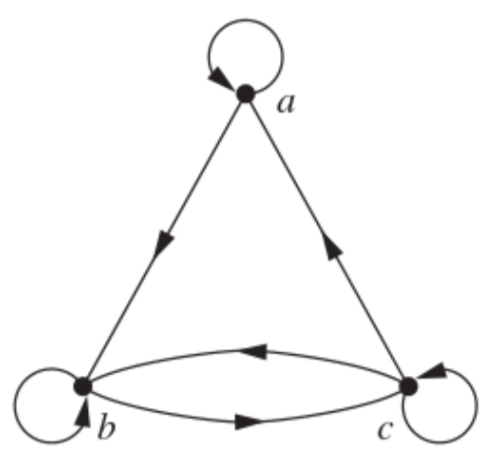
\includegraphics[height=4cm]{6-1.PNG}\\
  \end{center}
  \end{figure}
  
  
  R is reflexive if all elements point to themselves. $\{(a,a), (b,b), (c,c)\}$ all exist in R so R is reflexive. \\
  R is symmetric if all pairs point to each other. $\{(b,a), (a,c)\}$ do not exist in R so R is not symmetric. \\
  R is antisymmetric if all pairs are unmatched and there is all or none of the $a=b$ pairs. R is not symmetric, but it also contains all three of $\{(a,a), (b,b), (c,c)\}$ meaning that R is antisymmetric. \\
  R is transitive if $\{(a,b)$ and $(b,c)$ then $(a,c)\}$. $(c,a)$ and $(a,b)$ exist and so does $(c,b)\therefore$ R is transitive. \\


    \item (25 pts) Let $R=\{(1,2),(2,3),(3,4),(2,1)\}$ on set $A=\{1,2,3,4\}$. What is $R^2$ and $R^3$\\
    	\tab $R^2 = \{(1,3), (2,4), (1,1), (2,2)\} $\\
	\tab $R^3 = \{(1,4), (2,3)\} $ \\\\

  
    \item (40 pts) Let $R = \{(1,3),(1,4),(2,1),(2,2),(3,1),(3,3),(4,1)\}.$ on set $A=\{1,2,3,4\}$. 
\begin{itemize}
  \item What is the matrix representation of R?
    \[\begin{bmatrix}
	0 & 0 & 1 & 1  \\
	1 & 1 & 0 & 0  \\
	1 & 0 & 1 & 0  \\
	1 & 0 & 0 & 0  \\
    \end{bmatrix}\]
  \item What is the digraph representation of R?
  
    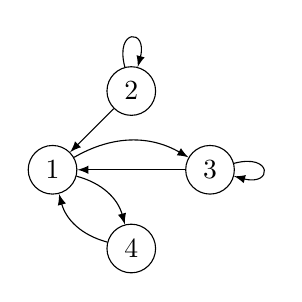
\begin{tikzpicture}
	\tikzset{vertex/.style = {shape=circle,draw,minimum size=1.5em}}
	\tikzset{edge/.style = {->,> = latex}}
	% vertices
	\node[vertex] (a) at  (-1, 0) {$1$};
	\node[vertex] (b) at  (0,1) {$2$};
	\node[vertex] (c) at  (1,0) {$3$};
	\node[vertex] (d) at  (0,-1) {$4$};
	%edges
	\draw[edge] (a) to[bend left] (c);
	\draw[edge] (a) to[bend left] (d);
	\draw[edge] (b) to (a);
	\draw[edge] (b) to[loop above] (b);
	\draw[edge] (c) to (a);
	\draw[edge] (c) to[loop right] (c);
	\draw[edge] (d) to[bend left] (a);
    \end{tikzpicture}
	
  \item What is the reflexive closure of $R$? \\
  	\tab All of $R$ plus the values that make it reflexive:\\
  	\tab $\{(1,3),(1,4),(2,1),(2,2),(3,1),(3,3),(4,1), (1,1), (4,4) \}$ \\
  \item What is the symmetric closure of $R$ \\
  	\tab All of $R$ plus the values that make it symmetric:\\
  	\tab $\{ (1,3),(1,4),(2,1),(2,2),(3,1),(3,3),(4,1),(1,2) \}$ \\
\end{itemize}

 \end{enumerate}

\end {document}
